\chapter{Energy balance with thermodynamic tabulations}
%\chaptermark{Energy Balance with thermodynamic tabulations}
\begin{nolinkcolors} 
\minitoc
\end{nolinkcolors}
\newpage
%
%
%=====================================
\section{State of the art}
%=====================================
\comment{ Use of enthalpy resolution in the majority of works \\
 motivation and advantages of TvsH without talking about resolution time\\
 use article's introduction to fill this section (or improvise new things)}
%
When speaking about macrosegregation, one needs to know that the problem involves phase change.
For that, a minimum of four conservation equations are necessary:
conservation  of  mass, momentum,  chemical  species and  energy. The  phase  change
literature  contains a  wealth of numerical methods to solve energy conservation
in solidifying alloys. A comprehensive overview of these methods is given by \citet{swaminathan._enthalpy_1993}.
The corresponding equation associates the total average enthalpy to the
temperature  via  intrinsic  alloy  properties, such  as the heat  capacity of  the
phases and the latent  heat associated with the phase transformations. However, in the course
of solidification and while macrosegregation is taking place, these  properties may change because the average
composition may  vary  significantly: the  transformation paths are thus modified, as well as
the phases' composition and heat capacity. Similarly, the latent heat of phase  transformations
is  not a mere constant that could be distributed as a function of the phase fractions
assuming only temperature-dependent phases' properties, as often found in the literature \citep{bellet_call_2009}.
It is thus impossible to establish a priori the dependence of the enthalpy with respect
to temperature when macrosegregation takes place, even in the case of full thermodynamic equilibrium
between phases. In this chapter, we discuss a suitable numerical scheme based on an enthalpy method,
already used in the literature  to  alleviate this macrosegregation-related problem \citep{swaminathan._enthalpy_1993,
carozzani_direct_2013}. Later on, we introduce a modified formulation, using the effective heat capacity method that 
increases the original scheme's efficiency. 

The current method is thus an enthalpy method that makes use of a temperature-based solver. 
Moreover, it uses tabulated thermodynamic quantities (solidification paths, phases' enthalpy  and composition) 
in a range of average compositions and temperatures as found in the literature 
\citep{dore_modelling_2000,thuinet_prediction_2004,du_modeling_2007}, 
with the aim of evaluating the total average enthalpy as well as the effective heat capacity. 
The novelty of the modified method resides in the use of thermodynamic tabulations without losing 
the advantages of the previous method, thus yielding faster computation times while maintaining a 
good accuracy.
%
%
%=====================================
\section{Thermodynamic considerations}
%=====================================
%
%-----------------------------
\subsection{Volume averaging} 
%-----------------------------
\comment{the following paragraph will be deleted once the volume averaging has been introduced in chapter 1}
\red{A volume averaging technique was suggested to deal with the presence of multiple 
phases \citep{ni_volume-averaged_1991}. It locally considers a Representative Volume Element 
(RVE) that contains a single or several phases (these are not necessarily in thermodynamic equilibrium) 
at a mesoscopic scale. We represent, for each unknown $\psi$, an intrinsic volume average, $\avg{\psi}^{\phi}$ (also denoted $\avg{\psi^{\phi}}^{\phi}$ in the 
literature), corresponding to a phase $\phi$. 
The volume average $\avg{\psi}$ for this unknown in the RVE, hence averaged over all the present phases writes:}
%%-------------
\begin{align}
\label{eq:volume_average_psi}
& \avg{\psi} = \sum_\phi \gphi \avg{\psi}^{\phi}
\end{align}
%%-------------
where $g^\phi$ denotes the volume fraction of phase $\phi$ in the RVE. 
It should be emphasized that the averaging technique applies to virtually all thermodynamic variables (enthalpy, density $\dots$). 
Among these variables, the temperature is also considered to be uniform in the RVE. 
Applying the volume averaging technique to the energy 
conservation principle along with interfacial balances between the phases, results in the following averaged equation \citep{rappaz_numerical_2003}:
%%-------------
\begin{align}
\label{eq:averaged_energy_eqn}
& \frac{\d \rh}{\d t} + \nabvec \cdot \rhv = \nabvec \cdot \brac{\avg{\kappa} \nabvec T} + \avg{\dot{Q}_V}
\end{align}
%%-------------
where $\rho$ stands for the density, $h$ the mass enthalpy, $\vec{v}$ the velocity field, $\kappa$ the thermal conductivity, $T$ the temperature 
and $\dot{Q}_V$ a possible volume heat source. 
\Cref{eq:averaged_energy_eqn} is the standard averaged form of the energy conservation equation used in non-stationary phase 
change problems. 
\comment{ I could elaborate more in this paragraph by showing the possible equations for the explicit formulation and maybe a figure to show the AlSi7
computation that i did with a v small time step }
 
Once the variational form has been discretized in space and time, two possible resolution schemes emerge: the first is an 
explicit forward Euler scheme which gives rise to a linear equation where the temperature is known at time $t$, $T^t$. This requires very small 
time steps in the current context, which limits the solver’s usability at the scale of industrial applications. The second scheme is the 
backward Euler or full implicit discretization where terms are function of $T^{t+\Delta t}$. It leads to a nonlinear equation with 2 interdependent 
unknowns, $\rh^{t+\Delta t}$ and  $T^{t+\Delta t}$. It is clear that the nature of the temperature-enthalpy relationship plays a central 
role when formulating the resolution strategy of this nonlinear equation. Generally, it is admitted that, depending on the resolution strategy, 
it is necessary to express enthalpy as a function of temperature or vice-versa, together with associated partial derivatives, 
$\frac{d \rh}{dT}$ or $\frac{dT }{d \rh}$.

\subsection{The temperature-enthalpy relationship} 
In solidification problems, additional variables are involved in \cref{eq:volume_average_psi} and \cref{eq:averaged_energy_eqn}, 
like the transformation path that defines the history of the phase fractions, as well as the average chemical composition $\wi$, 
i being the index of the chemical species (only the solutes are considered). The temperature-enthalpy relation averaged over the 
phases in a given RVE writes:
%%-------------
\begin{align}
\label{eq:volume_average_enthalpy}
& \rh = \sum_\phi \gphi_{\brac{T, \wi \dots}} \rphi_{\brac{T, \wi^{\phi} \dots}} \hphi_{\brac{T, \wi^{\phi} \dots}}
\end{align}
%%-------------
Note that the volume average enthalpy is approximated by the product $\avg{\rho h}^{\phi}=\avg{\rho}^{\phi}\avg{h}^{\phi}$ in the current work. As stated 
in the introduction, it becomes clear from \cref{eq:volume_average_enthalpy} that phase properties, i.e. average phase density, , \rphi and enthalpy, \hphi, 
are temperature and composition dependent. This equation is the key to convert the average volume enthalpy to temperature (through a procedure named \HtoT) 
or vice-versa (\TtoH). The values of the different phase fractions $\gphi$ (solidification path) and phase enthalpies $\rh^{\phi}$ are thus needed 
to close the relation.

\subsection{Tabulation of properties}
The complexity of performing a thermodynamic conversion is directly linked 
to the simplicity of determining the alloy properties, namely the phase fractions 
and phase enthalpies. In the case of binary alloys and with several assumptions 
with respect to the system (e.g., linear monovariant temperature composition 
relationships, constant heat capacity of phases and constant latent heat of transformations, 
equilibrium approximations between phases) analytical calculations are often used to determine 
the properties. Nevertheless, analytical relations are more complex or even impossible to derive 
in the case of multicomponent alloys ($i>1$). To overcome this problem, one can resort to 
thermodynamic databases and phase equilibrium calculations to tabulate the transformation paths 
and the phase enthalpies for a given range of temperatures and average compositions. It is a handy 
solution for two main reasons: first, the conversion is merely a binary search in a table; secondly, 
it is a simple solution for coupling with macrosegregation. In this way, phase fractions $\gphi$ are 
tabulated as functions of temperature and average composition, while for each phase $\phi$ the mass 
enthalpy, $\hphi$, and the density, $\rphi$, are tabulated as functions of temperature and phase 
intrinsic average compositions $\wiphi$, as well as other possible parameters. \Cref{Table:t2h_data} summarizes the 
steps in order to perform a temperature-to-enthalpy (\TtoH) conversion using the predefined tabulation 
approach. In step 1, the transformation path is acquired for each average composition and temperature 
to determine the list of phases, their volume fractions $\gphi$ and their intrinsic compositions $\wi^{\phi}$. 
In step 2, the phase enthalpy $\hphi$  and density $\rphi$ are determined by searching for the temperature and 
the already known phase composition $\wi^{\phi}$. In step 3, the average volume enthalpy is computed from the 
volume fraction, density and mass enthalpy of phases using \cref{eq:volume_average_enthalpy}.
%
%---------------------------
% this table did not work when using custom tabulate env. because of the call to \cref ?
\begin{table}[htbp]
\centering
\caption{Tabulation processing for a \TtoH procedure}
\label{Table:t2h_data}
{\tabulinesep=1.0mm
\begin{tabu}{|c|c|c|c|}
\tabucline[1pt]{-}
\textbf{Step Number} 	& 	\textbf{1}	& \textbf{2}	& 	\textbf{3} 				\\\tabucline[1pt]{-}
\textbf{Inputs} 		&  ${T,\wi}$	& ${T,\wiphi}$	&	${\gphi, \rphi \hphi}$ \\
\textbf{Outputs} 		&  ${\gphi,\wiphi}$	& ${\rphi,\hphi}$	&	${\avg{\rho h}}$ (\cref{eq:volume_average_enthalpy})
				\\\tabucline[1pt]{-}
\end{tabu}}
\end{table}
%---------------------------
%
The methodology to build the tabulations is straightforward. It is based on two main scans. On the one hand, intervals for the variation of the 
average composition $\wi$ are chosen from the known alloy composition. These variations have to cover the extreme values adopted during the 
simulation, which are not known a priori. An interval is also selected for the variation of temperature. The latter is easier to determine as it
usually starts from the initial melt temperature and goes down to the room temperature in a standard casting simulation. For these intervals, a 
systematic scan is made with chosen steps in each composition and T, during which a thermodynamic equilibrium is computed. The outputs are the 
number of phases encountered, together with their fraction and intrinsic composition. The minimum and maximum intrinsic composition for each phase 
could then be determined. On the other hand, for each phase, a scan of the intrinsic composition and temperature is made to compute the intrinsic 
properties. The same temperature interval and step as defined earlier are used.

\comment{ below paragraph should be re written and maybe stress LESS on the speed effect}
\comment{ I should change the superscript $k$ which may be confused with partition coefficient }
Regarding the enthalpy-to-temperature conversion (\HtoT), a backward iterative \TtoH search is performed. 
For a known composition $\wi$, denoting $k$ the iteration index to convert the enthalpy 
$\avg{\rho h}_{\text{input}}$, we start with an initial guess for temperature $\Tkinit$ then convert it to an 
enthalpy  $\Hkinit$ with the \TtoH conversion. Using an appropriate nonlinear algorithm (Brent is the most versatile 
in our case), we aim at minimizing the following residual: $\text{Residu}_{\rh} = \abval{\rh_{\text{input}} - \Hk }$. 
Once the algorithm has converged, the temperature $\Tk$ is the result of the \HtoT conversion. It is 
inferred that the first conversion (\TtoH) is a direct one whereas the latter (\HtoT) is indirect and requires 
a series of iterative steps; each step being a single \TtoH resolution. In other words, a \HtoT conversion is a 
backward search for a temperature, hence it’s slower. This conversion’s speed lag is exacerbated when tabulations 
increase in size (e.g. large number of temperature and composition steps) and complexity (e.g., multicomponent 
industrial alloys used in casting), since the search gets more complicated with the increasing number of input 
columns (one column for each alloying element).
%
%
%==================
\section{Numerical method}
%==================
%
The finite element method is used to solve the energy conservation as expressed by \cref{eq:averaged_energy_eqn}. 
A test function $\test$ belonging to the Hilbertian Sobolev space $\hilbert(\Omega)$ of continuous integrable test functions 
is used to formulate the integral variational form of \cref{eq:averaged_energy_eqn} \citep{suli_lecture_2000}. 
A Fourier boundary condition is considered on the domain boundary $\partial \Omega$. The domain $\Omega$
is discretised using first-order linear simplexes defined by their number of local nodes (denoted “NbLoc”): triangles 
in 2D with NbLoc=3 and tetrahedra in 3D with  NbLoc=4. The outcome is a residual that we aim to minimize so that the 
conservation principle is satisfied. Therefore, the weak form writes:
%----------------------
\begin{multline}
\label{eq:weak_energy}
\forall \test \in M=\curly{u \in \hilbert(\OhmE)} \\
\integral{\OhmE}{\test \tempup{\rhoh}}{V} 
 + \integral{\OhmE}{\test \vit \cdot \nabvec \brac{\rhol \hl}}{V}
 - \integral{\OhmE}{\test \diff{\avg{\kappa}}{T} }{V}
 - \integral{\OhmE}{\test \source }{V}
 = 0
\end{multline}
%------------
where we assumed a static solid phase and an incompressible liquid phase, which allowed recasting the second term of 
\cref{eq:averaged_energy_eqn} into $\vit \cdot \nabvec \brac{\rhol \hl}$. 
The steps for discretizing in time and space the previous equation are well detailed in  some book references like \citet{rappaz_numerical_2003,dantzig_solidification_2009}. As for enthalpy and temperature, they are spatially discretized in each simplex 
using interpolations functions $\interp$, thus defining the nodal values $H_j$ and $T_j$, respectively: 
%----------------------
\begin{align}
\label{eq:discretise_H}
\rhoh 	&= \sum_{j=1}^{\text{NbLoc}}  \interp_j   \Hj \\ 
\label{eq:discretise_T}
T		&= \sum_{j=1}^{\text{NbLoc}}  \interp_j   \Tj
\end{align}
%------------
Note that $H_j$ is a volumetric enthalpy. The Galerkin formulation gives the following expression for the residual contribution at a mesh node $i$ for time step $t$ in a local element $\element$:
%----------------------
\begin{align}
\begin{split}
\label{eq:discretise_residual_local}
& \brac{R_i^E}^t = \Mij^E \brac{\Hjt - \Hjtminus} + \Aij^E \Tjt + \brac{\Kija^E + \Kijb^E}-\Fi^E - \Si^E=0 \\
& i,j:1 \rightarrow \text{NbLoc}
\end{split}
\end{align}
%------------
where the numerical contributions can be detailed as follows:
%----------------------
\begin{align}
& \textit{transient term:} \quad  \Mij^E = \integral{\OhmE}{\frac{1}{\dt} \interp_i \interp_j }{V} \\ 
& \textit{advection term:} \quad  \Aij^E = \integral{\OhmE}{\rhol \cpl \interp_i \vit \cdot \nabvec \interp_j}{V} \\ 
& \textit{diffusion term:} \quad  \Kija^E = \integral{\OhmE}{\avg{\kappa} \nabvec \interp_i\nabvec \interp_j}{V} \\ 
& \textit{boundary condition term 1:}	\quad  \Kijb^E = \integral{\dOhmE}{\hext \interp_i \interp_j}{S} \\ 
& \textit{boundary condition term 2:}	\quad	\Fi^E = \integral{\dOhmE}{\hext \Text \interp_i}{S} \\
& \textit{source term:} \quad  \Si^E = \integral{\OhmE}{\interp_i \source}{V}
\end{align}
%------------
%
The surface integrals $\Kijb^E$ and $\Fi^E$ are related to a Fourier-type boundary condition, 
with $\hext$ as a coefficient of heat exchange and $\Text$ as the external temperature far from the 
boundary. The energy conservation principle is satisfied when the sum of the residual contributions 
coming from all the mesh elements is zero. In other words, the following global residual defined by 
the assembly of these contributions, should be minimized: 
%----------------------
\begin{align}
\begin{split}
\label{eq:discretise_residual_global}
& \brac{R_i}^t = \Mij \brac{\Hjt - \Hjtminus} + \Aij \Tjt + \brac{\Kija + \Kijb}\Tjt -\Fi - \Si=0 \\
& i,j:1 \rightarrow \text{NbGlob}
\end{split}
\end{align}
%------------
where the global tensors $\Mij$, $\Aij$, $\Kija$ , $\Kijb$ , $\Fi$ and $\Si$ contain respectively, after an assembly step, 
the contributions of the local matrices $\Mij^E$, $\Aij^E$, $\Kija^E$ , $\Kijb^E$ , $\Fi^E$ and $\Si^E$ from each discretised 
element in the domain $\Ohm$. Accordingly, the indices $i$ and $j$ refer to global node numbers, where the total number of nodes is 
denoted by "NbGlob". It is clear that the global residual inherits the dependence between enthalpy and temperature. 
This is shown in \cref{eq:discretise_residual_global} where the average volume enthalpy is a function of the temperature. It infers that this residual 
is a non-linear function; therefore minimizing it requires an iterative non-linear algorithm. Our choice settles on the 
Newton-Raphson method, known for its quadratic convergence speed. A solidification problem can induce severe non-linearities 
from the release of the latent heat (which itself is temperature-composition dependent) and the variations of the thermophysical 
properties of the alloy with respect to temperature and average composition. This algorithm could thus treat such variations. 
Considering the link between enthalpy and temperature, \cref{eq:discretise_residual_global} may be solved either for enthalpy 
or for temperature as a nodal unknown; hence both formulations are presented hereafter.
%
%
%---------------
\subsection{Enthalpy-based approach }
%---------------
The residual is re-written using a Taylor series expansion to the first order for a nonlinear iteration $\iter$ :
%-----------------
\begin{align}
\label{eq:Hsolver_residual}
& \brac{R_i}^\iterplus = \brac{R_i}^\iter + \brac{\dRdH}^{\iter}_{ij} \Delta \Hj^\iter + \order\brac{\Hj^2}
\end{align}
%------------
Neglecting the second order terms, the suggested correction at each iteration in view of cancelling 
the residual and giving the new value $\Hj^\iter$, is given by the linear system in \cref{eq:Hsolver_residual_linear}
relative to what we call a \emph{Hsolver}:
%-----------------
\begin{align}
\label{eq:Hsolver_residual_linear}
& \brac{\dRdH}^{\iter}_{ij} \brac{\Hj^\iterplus - \Hj^\iter} = -R_i^\iter
\end{align}
%------------
where $\dRdH$ is a global tangent matrix yielding the variations of the residual with respect to the enthalpy 
in the last iteration, $\Hj^\iter$. If \cref{eq:discretise_residual_local} is considered, then the contribution of an element $\OhmE$ writes:
%-----------------
\begin{align}
\label{eq:dRdH}
& \brac{\dRdH}^{\iter E}_{ij} 
= \Mij^E 
+ \underbrace{\Aij^E \brac{\dTdH}^{\iter}_{j}}_{\nosum}
+ \underbrace{\brac{\Kija^E + \Kijb^E} \brac{\dTdH}^{\iter}_{j}}_{\nosum}
\end{align}
%------------
\Cref{eq:dRdH} is the core of the enthalpy-based solver. The resolution of \cref{eq:Hsolver_residual_linear} 
then yields a new estimate of the vector of nodal enthalpies $H^\iterplus$, which are the only unknowns to be solved for. 
Once determined at iteration $\iter$, convergence tests are performed (refer to section %TODO ).
%
%
%---------------
\subsection{Temperature-based approach }
%---------------
Similarly to the Hsolver, the local residual is recast for a nonlinear iteration $\iter$, 
leading this time to an iterative temperature correction:
%-----------------
\begin{align}
\label{eq:Tsolver_residual_linear}
& \brac{\dRdT}^\iter_{ij} \brac{\Tj^\iterplus - \Tj^\iter} = -R_i^\iter
\end{align}
%------------
where $\dRdT$ is a global tangent matrix yielding the variations of the residual with respect to temperature $\Tj^\iter$ at the previous iteration. 
This solver will be referred to as \emph{Tsolver}.
The contribution of an element $\OhmE$ to this tangent matrix is evaluated as:
%-----------------
\begin{align}
\label{eq:dRdT}
& \crochet{\dRdTijk}^E
= \underbrace{\Mij^E \brac{\dHdT}^{\iter}_{j}}_{\nosum}
+ \Aij^E
+ \brac{\Kija^E + \Kijb^E}
\end{align}
%------------
In contrast to the previous solver, \cref{eq:dRdT} is the core of the temperature-based solver. The resolution of \cref{eq:Tsolver_residual_linear} 
then yields a new estimate of the vector of nodal temperatures $T^\iterplus$, which are the only unknowns to be solved for. 
Once updated for iteration $\iter$, convergence tests are performed (refer to section %TODO ).
%
%
%-------------------
\subsection{Convergence}
%
The previous two sections described the iterative resolution of the same discretised energy 
conservation by both Tsolver and Hsolver. However, in \cref{eq:dRdH,eq:dRdT}, an important 
term emerges from the tangent matrix evaluation describing the variations between temperature 
and enthalpy: $\dHdT$ (or $\dTdH$). This term invokes the previously mentioned temperature-enthalpy 
tabulations which depend on the alloy composition. Consequently,  $\dHdT$ (or $\dTdH$)
has a great influence on the convergence of the Tsolver (respectively the Hsolver). 
When \cref{eq:Hsolver_residual_linear} or \cref{eq:Tsolver_residual_linear} is solved at iteration $\iter$, this term is written using a finite difference:
%-----------------
\begin{align}
\label{eq:finite_difference_Tsolver}
& \textbf{Tsolver} \qquad \brac{\dHdT}^{\iterplus}_{j} = \frac{\rhoh_j^\iterplus - \rhoh_j^\iter}{T_j^\iterplus - T_j^\iter} \\
\label{eq:finite_difference_Hsolver}
& \textbf{Hsolver} \qquad \brac{\dTdH}^{\iterplus}_{j} = \frac{T_j^\iterplus - T_j^\iter}{\rhoh_j^\iterplus - \rhoh_j^\iter}
\end{align}
%------------
For the Tsolver, the enthalpy $\rhoh_j^\iter$ is needed to evaluate \cref{eq:finite_difference_Tsolver}. 
In contrast, the Hsolver requires the value of $T_j^\iter$ to evaluate the corresponding \cref{eq:finite_difference_Hsolver}.
In both cases, the unknown is determined by the temperature-enthalpy relation. The indices next to the mentioned unknowns
indicate that this relation is used for each iteration $\iter$ at each mesh node $j$, hence affecting the global resolution time 
between the two solvers. The Hsolver needs a \HtoT to evaluate $\dTdH$, whereas the Tsolver needs a \TtoH to evaluate $\dHdT$. 
The flowchart in \cref{fig:} demonstrates the process.
It can be seen that Tsolver uses solely \TtoH procedure and the thermodynamic tabulations to determine the enthalpy, 
hence the term $\dHdT$. On the other hand, Hsolver repeats the same procedure a finite number of times in order to 
determine a temperature output through \HtoT and use it to compute $\dTdH$. This algorithmic difference leverages the 
Tsolver in terms of computation time providing the same numerical accuracy while conserving the total system energy. 
%
%---------------
\begin{figureth}
% textwidth 
{0.65}
%path 
{Misc/dummy.pdf}
% caption
{Flowcharts showing the steps to compute the nonlinear terms using tabulations}
% label
\label{fig:diagram}
\end{figureth}
%==================
%
Convergence tests are necessary at the end of each iteration of the energy solver to determine 
the convergence status of the algorithm. In the context of the Tsolver for instance, the residual 
is re-evaluated with the newly determined temperature $\Tj^\iterplus$ and enthalpy $\Hj^\iterplus$ so \cref{eq:discretise_residual_global} rewrites:
%-----------------
\begin{align}
\begin{split}
\label{eq:discretise_residual_global_new}
& \brac{R_i}^\iterplus = \Mij \brac{\Hj^\iterplus) - \Hjtminus} + \Aij \Tj^\iterplus + \brac{\Kija + \Kijb}\Tj^\iterplus -\Fi - \Si \\
& i,j:1 \rightarrow \text{NbGlob}
\end{split}
\end{align}
%------------
The norm of the current residual, $\norm{R^\iterplus}$, is compared to a fixed small 
value $\varepsilon_R \approx \crochet{\num{d-5};\num{d-4}}$. The resulting temperature variation, 
$\abval{\Tj^\iter-\Tj^\iterminus}$, should also respond to similar criterion between two consecutive 
iterations. For that purpose, we compare it to another fixed value $\varepsilon_T \approx \crochet{\num{d-3};\num{d-2}}$.
Convergence is ultimately achieved when the following criteria are simultaneously met:
%------
\begin{equation}
\label{eq:energy_convergence_criteria}
   \left\{
   \begin{aligned}
      & \norm{R^\iterplus} < \varepsilon_R \\
	  & \text{Max}_{j:1 \rightarrow \text{NbGlob}} \abval{\Tj^\iterplus-\Tj^\iter} < \varepsilon_T
    \end{aligned}
    \right.
\end{equation}
%------------
A comparison of both solver formulations is done in the hereafter test cases section.
%
%
%
\begin{figure}[htbp]
%\newlength{\largeur}	% defined in chapter2
%\newlength{\llargeur}	% defined in chapter2
%\newlength{\rlargeur}	% defined in chapter2

\setlength{\largeur}{13.5cm}
\setlength{\llargeur}{3.8cm}
\centering
\begin{tikzpicture}[node distance=0.3cm]

\tikzstyle{rect}=[rectangle,draw,text=black]
\tikzstyle{whiterect}=[rectangle,text=black]
\tikzstyle{test}=[diamond,aspect=3,draw,text=black]
\tikzstyle{fleche}=[->,>=stealth]
\tikzstyle{trait}=[]

\setlength{\rlargeur}{\largeur}
\addtolength{\rlargeur}{-2.\tabcolsep}
\addtolength{\rlargeur}{-1.\llargeur}


\node[rect] (init) at (0cm,5cm)
{
	\begin{tabular}{@{}p{\llargeur}p{\rlargeur}@{}}
		\textbf{Initialisation} \\
		Time stepping 	& $t$, $\Delta t$ \\
		Nodal values	& $\Hjt$, $\Tjt$, $\dHdTjt$ %, $\avg{w}^t$, $\avg{v^l}^t$
	\end{tabular}
};

\node[rect,below=of init] (init_iter)
{
	\begin{tabular}{@{}p{\llargeur}p{\rlargeur}@{}}
		\textbf{Newton-Raphson} \\		
		Iteration step	& $\iter=0$ \\
		Nodal values 	& $\Hjk=\Hjt$, \\ 
						& $\Tjk=\Tjt$, \\
						& $\dHdTjk=\dHdTjt$ %, $\avg{w}^t$, $\avg{v^l}^t$
	\end{tabular}
};
	
\node[rect,below=of init_iter] (local_contrib)
{
	\begin{tabular}{@{}p{\llargeur}p{\rlargeur}@{}}
		\textbf{Local contributions} \\
		& $\crochet{A_{ij}^\iter}^E=\crochet{\dRdTijk}^E$  \quad (\cref{eq:dRdT}) \\
		& $\crochet{b_{j}^\iter}^E=\crochet{\dRdTijk}^E \Tjk - \Rjk$	\quad (\cref{eq:discretise_residual_local})
	\end{tabular}
};

\node[rect,below=of local_contrib] (assembly)
{
	\begin{tabular}{@{}p{\llargeur}p{\rlargeur}@{}}
	\textbf{Matrices assembly}\\
		Global matrices & 	$\crochet{A^\iter} \leftarrow \crochet{A^\iter}^E$, $\crochet{b^\iter} \leftarrow \crochet{b^\iter}^E$, $\forall E \in \Ohm$ \\
		Residual norm	&	$\norm{R^\iter} = \norm{A^\iter \Tk - b^\iter}$ \\ 
	\end{tabular}
};

\node[rect,below=of assembly] (solve)
{
	\begin{tabular}{@{}p{\llargeur}p{\rlargeur}@{}}
	\textbf{Solve linear system} &	$ \Tkplus= (A^\iter)^{-1} b^\iter$ \\
	\end{tabular}
};


\node[rect,below=of solve] (microseg)
{
	\begin{tabular}{@{}p{\llargeur}p{\rlargeur}@{}}
	\textbf{Microsegregation} \\
	Tabulation (\TtoH) 	&	$ \rhoh^\iterplus=\sum_\phi \crochet{\gphi \rphi \hphi}_{T=\Tkplus}$ \quad (\cref{eq:volume_average_enthalpy})\\
	Update				& 	$\dHdTjkplus=f(\Tjkplus,\rhoh^\iterplus)$ (\cref{eq:finite_difference_Tsolver})\\
	\end{tabular}
};

\node[rect,below=of microseg] (reassembly)
{
	\begin{tabular}{@{}p{\llargeur}p{\rlargeur}@{}}
	\textbf{Matrices reassembly}\\
		Global matrices & 	$\crochet{A^\iterplus} \leftarrow \crochet{A^\iterplus}^E$, $\crochet{b^\iterplus} \leftarrow \crochet{b^\iterplus}^E$, $\forall E \in \Ohm$ \\
		Residual norm	&	$\norm{R^\iterplus} =  \norm{A^\iterplus \Tkplus - b^\iterplus}$ \\ 
	\end{tabular}
};

\node[test,below=of reassembly,shift={(-3.7cm,0mm)}] (convergence_res)
{
	\begin{tabu}{c}
	$\norm{R^\iterplus} < \varepsilon_R $ \\
	%Max $\Delta T_j < \varepsilon_T$ \\
	(\cref{eq:energy_convergence_criteria})
	\end{tabu}
};


\node[test,right=of convergence_res,shift={(0.2cm,0mm)}] (convergence_temp)
{
	\begin{tabu}{c}
	%$\norm{R^\iterplus} < \varepsilon_R $ \\
	Max $\Delta T_j < \varepsilon_T$ \\
	(\cref{eq:energy_convergence_criteria})
	\end{tabu}
};


\node[rect,below=of reassembly,shift={(0.0cm,-3cm)}] (update)
{
	\begin{tabular}{@{}p{\llargeur}p{\rlargeur}@{}}
	\textbf{Update} &	\\
	Nodal values	& $\Hjtplus=\Hjkplus$, $\Tjtplus=\Tjkplus$ \\
	\end{tabular}
};

\node[test,below=of update, aspect=4] (test_end)
{
	$t+\dt=t_{end}$
};



\node[rect,right=of test_end] (end)
{
	End
};

\draw[trait] (init) -- (init_iter);
\draw[trait] (init_iter) -- (local_contrib);
\draw[trait] (local_contrib) -- (assembly);
\draw[trait] (assembly) -- (solve);
\draw[trait] (solve) -- (microseg);
\draw[trait] (microseg) -- (reassembly);
%\draw[trait] (reassembly.south) -- (convergence_res.north);
\draw[trait] (convergence_res) -- (convergence_temp);
%\draw[trait] (convergence_temp.south) -- (update.north);
\draw[trait] (update) -- (test_end);
\draw[trait] (test_end) -- (end);

\coordinate[shift={(0mm,-2mm)}] (convsouth) at (convergence_res.south);
\coordinate[shift={(-8mm,0mm)}] (contribwest) at (local_contrib.west);
\draw[fleche] (convergence_res.south) -- (convsouth) -| (contribwest) -- (local_contrib.west);

\coordinate[shift={(0mm,-2mm)}] (reassemblysouth) at (reassembly.south);
\draw[trait] (reassembly.south) -- (reassemblysouth) -| (convergence_res);

\coordinate[shift={(0mm,-2mm)}] (convergence_tempsouth) at (convergence_temp.south);
\coordinate[shift={(-8mm,0mm)}] (contribwest_bis) at (local_contrib.west);
\draw[trait] (convergence_temp.south) -- (convergence_tempsouth) -| (contribwest_bis.west) -- (local_contrib);

\coordinate[shift={(2mm,0mm)}] (convergence_tempeast) at (convergence_temp.east);
\coordinate[shift={(0mm,2mm)}] (updatenorth) at (update.north);
\draw[trait] (convergence_temp.east) -- (convergence_tempeast) |- (updatenorth) -- (update);

\coordinate[shift={(-12mm,0mm)}] (initwest) at (init.west);
\draw[fleche] (test_end.west) -| (initwest) -- (init);

%%-------------
\coordinate[shift={(6mm,0mm)}] (convsouth_no) at (convsouth.east);
\node[anchor=south west] (convres_no) at (convsouth_no.east) {No};
\coordinate[shift={(6mm,0mm)}] (convsouthtemp_no) at (convergence_tempsouth.east);
\node[anchor=south west] (convtemp_no) at (convsouthtemp_no.east) {No};
\coordinate[shift={(-1.2cm,0mm)}] (convsouth_process) at (convsouth.west);
\node[anchor=south east] (conv_no_process) at (convsouth_process.west) {$\iter \leftarrow \iterplus$};
%%-------------
\node[anchor=south east] (test_end_no) at (test_end.west) {No};
\node[anchor=north east] (test_end_process) at (test_end.west) {$t \leftarrow t+\dt$};
%%-------------

\end{tikzpicture}

\caption{Resolution algorithm of the temperature-based solver.}

\end{figure}
%
%
%
%
%
\begin{figure}[htbp]

\setlength{\largeur}{13.5cm}
\setlength{\llargeur}{3.8cm}
\centering
\begin{tikzpicture}[node distance=0.3cm]

\tikzstyle{rect}=[rectangle,draw,text=black]
\tikzstyle{whiterect}=[rectangle,text=black]
\tikzstyle{test}=[diamond,aspect=3,draw,text=black]
\tikzstyle{fleche}=[->,>=stealth]
\tikzstyle{trait}=[]

\setlength{\rlargeur}{\largeur}
\addtolength{\rlargeur}{-2.\tabcolsep}
\addtolength{\rlargeur}{-1.\llargeur}

\node[rect] (init) at (0cm,5cm)
{
	\begin{tabular}{@{}p{\llargeur}p{\rlargeur}@{}}
		\textbf{Initialisation} \\
		Time stepping 	& $t$, $\Delta t$ \\
		Nodal values	& $\Hjt$, $\Tjt$, $\dTdHjt$ %, $\avg{w}^t$, $\avg{v^l}^t$
	\end{tabular}
};

\node[rect,below=of init] (init_iter)
{
	\begin{tabular}{@{}p{\llargeur}p{\rlargeur}@{}}
		\textbf{Newton-Raphson} \\		
		Iteration step	& $\iter=0$ \\
		Nodal values 	& $\Hjk=\Hjt$, \\ 
						& $\Tjk=\Tjt$, \\
						& $\dTdHjk=\dTdHjt$ %, $\avg{w}^t$, $\avg{v^l}^t$
	\end{tabular}
};
	
\node[rect,below=of init_iter] (local_contrib)
{
	\begin{tabular}{@{}p{\llargeur}p{\rlargeur}@{}}
		\textbf{Local contributions} \\
		& $\crochet{A_{ij}^\iter}^E=\crochet{\dRdHijk}^E$  \quad (\cref{eq:dRdH}) \\
		& $\crochet{b_{j}^\iter}^E= \Rjk$	\quad (\cref{eq:discretise_residual_local})
	\end{tabular}
};

\node[rect,below=of local_contrib] (assembly)
{
	\begin{tabular}{@{}p{\llargeur}p{\rlargeur}@{}}
	\textbf{Matrices assembly}\\
		Global matrices & 	$\crochet{A^\iter} \leftarrow \crochet{A^\iter}^E$, $\crochet{b^\iter} \leftarrow \crochet{b^\iter}^E$, $\forall E \in \Ohm$ \\
		Residual norm	&	$\norm{R^\iter} =  \norm{A^\iter \deltaHk - b^\iter}$ \\ 
	\end{tabular}
};

\node[rect,below=of assembly] (solve)
{
	\begin{tabular}{@{}p{\llargeur}p{\rlargeur}@{}}
	\textbf{Solve linear system} &	$ \Delta \Hkplus= (A^\iter)^{-1} b^\iter$ \\
	\textbf{Update iterate} &	$ \Hjkplus = \Delta \Hjkplus + \Hjk$ \\
	\end{tabular}
};


\node[rect,below=of solve] (microseg)
{
	\begin{tabu}{@{}p{\llargeur}p{\rlargeur}@{}}
	\textbf{Microsegregation} \\
	Tabulation (\HtoT)	&	$ \rhoh^\iterplus \rightarrow \Tkplus$ \quad (Brent algorithm) \\
	Update				& 	$\dTdHjkplus=f(\Tjkplus,\rhoh^\iterplus)$ (\cref{eq:finite_difference_Hsolver})\\
	\end{tabu}
};

\node[rect,below=of microseg] (reassembly)
{
	\begin{tabular}{@{}p{\llargeur}p{\rlargeur}@{}}
	\textbf{Matrices reassembly}\\
		Global matrices & 	$\crochet{A^\iterplus} \leftarrow \crochet{A^\iterplus}^E$, $\crochet{b^\iterplus} \leftarrow \crochet{b^\iterplus}^E$, $\forall E \in \Ohm$ \\
		Residual norm	&	$\norm{R^\iterplus} =  \norm{A^\iterplus \deltaHkplus - b^\iterplus}$ \\ 
	\end{tabular}
};

\node[test,below=of reassembly,shift={(-3.7cm,0mm)}] (convergence_res)
{
	\begin{tabu}{c}
	$\norm{R^\iterplus} < \varepsilon_R $ \\
	%Max $\Delta T_j < \varepsilon_T$ \\
	(\cref{eq:energy_convergence_criteria})
	\end{tabu}
};


\node[test,right=of convergence_res,shift={(0.2cm,0mm)}] (convergence_temp)
{
	\begin{tabu}{c}
	%$\norm{R^\iterplus} < \varepsilon_R $ \\
	Max $\Delta T_j < \varepsilon_T$ \\
	(\cref{eq:energy_convergence_criteria})
	\end{tabu}
};


\node[rect,below=of reassembly,shift={(0.0cm,-3cm)}] (update)
{
	\begin{tabular}{@{}p{\llargeur}p{\rlargeur}@{}}
	\textbf{Update} &	\\
	Nodal values	& $\Hjtplus=\Hjkplus$, $\Tjtplus=\Tjkplus$ \\
	\end{tabular}
};

\node[test,below=of update, aspect=4] (test_end)
{
	$t+\dt=t_{end}$
};



\node[rect,right=of test_end] (end)
{
	End
};

\draw[trait] (init) -- (init_iter);
\draw[trait] (init_iter) -- (local_contrib);
\draw[trait] (local_contrib) -- (assembly);
\draw[trait] (assembly) -- (solve);
\draw[trait] (solve) -- (microseg);
\draw[trait] (microseg) -- (reassembly);
%\draw[trait] (reassembly.south) -- (convergence_res.north);
\draw[trait] (convergence_res) -- (convergence_temp);
%\draw[trait] (convergence_temp.south) -- (update.north);
\draw[trait] (update) -- (test_end);
\draw[trait] (test_end) -- (end);

\coordinate[shift={(0mm,-2mm)}] (convsouth) at (convergence_res.south);
\coordinate[shift={(-8mm,0mm)}] (contribwest) at (local_contrib.west);
\draw[fleche] (convergence_res.south) -- (convsouth) -| (contribwest) -- (local_contrib.west);

\coordinate[shift={(0mm,-2mm)}] (reassemblysouth) at (reassembly.south);
\draw[trait] (reassembly.south) -- (reassemblysouth) -| (convergence_res);

\coordinate[shift={(0mm,-2mm)}] (convergence_tempsouth) at (convergence_temp.south);
\coordinate[shift={(-8mm,0mm)}] (contribwest_bis) at (local_contrib.west);
\draw[trait] (convergence_temp.south) -- (convergence_tempsouth) -| (contribwest_bis.west) -- (local_contrib);

\coordinate[shift={(2mm,0mm)}] (convergence_tempeast) at (convergence_temp.east);
\coordinate[shift={(0mm,2mm)}] (updatenorth) at (update.north);
\draw[trait] (convergence_temp.east) -- (convergence_tempeast) |- (updatenorth) -- (update);

\coordinate[shift={(-12mm,0mm)}] (initwest) at (init.west);
\draw[fleche] (test_end.west) -| (initwest) -- (init);

%%-------------
\coordinate[shift={(6mm,0mm)}] (convsouth_no) at (convsouth.east);
\node[anchor=south west] (convres_no) at (convsouth_no.east) {No};
\coordinate[shift={(6mm,0mm)}] (convsouthtemp_no) at (convergence_tempsouth.east);
\node[anchor=south west] (convtemp_no) at (convsouthtemp_no.east) {No};
\coordinate[shift={(-1.2cm,0mm)}] (convsouth_process) at (convsouth.west);
\node[anchor=south east] (conv_no_process) at (convsouth_process.west) {$\iter \leftarrow \iterplus$};
%%-------------
\node[anchor=south east] (test_end_no) at (test_end.west) {No};
\node[anchor=north east] (test_end_process) at (test_end.west) {$t \leftarrow t+\dt$};
%%-------------

\end{tikzpicture}

\caption{Resolution algorithm of the enthalpy-based solver.}

\end{figure}
%
%
%

\section{Validation}
%==================
%
%------------------------------
\subsection{Pure diffusion}
%------------------------------
The two solvers are first tested in a purely diffusive case for a one-dimensional solidification configuration. 
Predictions with a 1D front tracking model \citep{gandin_constrained_2000} is used as a benchmark. It provides 
solutions for the temperature and solid fraction during directional solidification of a 10 cm long \bin{Al}{7}{Si}
ingot. The melt, with initial uniform temperature, is cooled with a heat exchange coefficient (assuming a Fourier 
boundary condition) from one side, the other side being adiabatic. All values for alloy properties, initial and 
boundary conditions and numerical parameters are listed in \cref{table:data_case_alsi7}. For this simple test case, 
we use linear temperature dependence of the intrinsic phase enthalpies, that is $\rh^s= \rcp T$ and $\rh^l= \rcp T + \rho L$, 
where $\rcp$ is the heat capacity per unit volume and $\rho L$ is the latent heat per unit volume. Values for $\rcp$ 
and $\rho L$, as well as for the thermal conductivities, $\kappa = \kl = \ks$, are taken constant. Moreover, a 
Gulliver Scheil approximation is used to compute a single temperature – fraction of solid relationship in the 
absence of macrosegregation. This is done assuming a linear binary phase diagram and thus requires using the 
properties listed in \cref{table:data_case_alsi7}, i.e. the segregation coefficient, $k$, the liquidus slope, $m_L$, the 
liquidus temperature, $T_L$, and the eutectic temperature, $T_E$. \Cref{fig:diffusion_CC,fig:diffusion_LF} show the comparison with 
the Hsolver and Tsolver. The results are found superimposed to the front tacking solution, thus giving validation 
of the implementation as well as the iterative schemes presented above to solve the energy conservation 
%------------------------
\begin{tabulate}
% caption 
{Parameters for the pure diffusion test case with an \bin{Al}{7}{Si} alloy presented in \cref{fig:diffusion_CC}}
% label
{table:data_case_alsi7}
% line separation (e.g. 1.5mm)
{1.0mm}
% column justification-number (e.g. |c|ll|)
{llll}
% header titles (should use the & sign to switch columns)
{\textbf{Parameter} & \textbf{Symbol} & \textbf{Value} & \textbf{Unit}}
% cells content (should use the & and // to switch columns and rows)
{Nominal composition 	& $\avg{w}_0$ & \num{7} & \si{\ucomposition} \\ 
Liquidus temperature 	& $T_L$ & \num{618} 	& \si{\udegC} \\ 
Eutectic temperature 	& $T_E$ & \num{577}	 	& \si{\udegC} \\  
Segregation coefficient & $k$ & \num{0.13} 		& $-$  \\  
Liquidus slope & $m_L$ 	& \num{-6.5} 			& \si{\uslope} \\ 
Heat capacity (liquid and solid) & $\rho C_p$ & \num{2.6e6} & \si{\uvolumecapacity} \\  
Enthalpy of fusion 				  & $\rho L$ & \num{9.5e8} 	& \si{\uvolumeenergy} \\ 
Thermal conductivity (liquid and solid) 	& $\kappa$ & \num{70} & \si{\uconductivity}	\\
\hline  
Heat transfer coefficient & $\hext$ & \num{500} & \si{\uhconvec} \\ 
External temperature 		& $\Text$ & \num{100} & \si{\udegC} \\ 
Initial temperature 		& $T_0$ & \num{800} & \si{\udegC} \\ 
Ingot length 				&  & \num{0.1} & \si{\metre} \\ 	
\hline 
FE mesh size 						&  					& \num{e-3} & \si{\metre} \\ 
Time step 							& $\dt$ 			& \num{0.1} & \si{\second} \\ 
Convergence criterion (residual) 	& $\varepsilon_R$	& \num{e-6} & $-$ \\ 
Convergence criterion (temperature) & $\varepsilon_T$ 	& \num{e-2} & \si{\udegK}}
%
\end{tabulate}
%------------------------
%
%-----------------
\begin{figure}[htbp]
\centering
   %------------
  \begin{subfigure}[t]{0.7\textwidth}
    \centering
	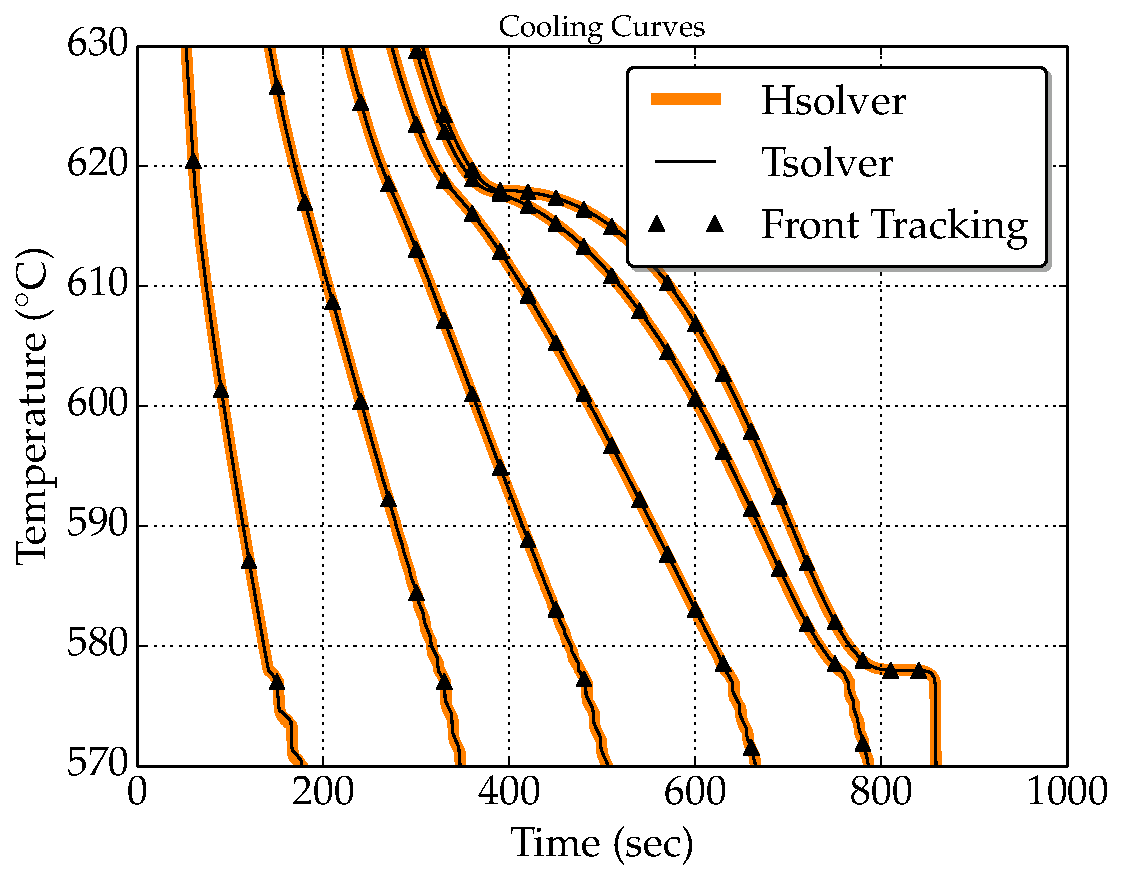
\includegraphics[width=\textwidth]{Chapter2/Graphics/diffusion/diffusion_CC.pdf}
	\caption{}
    \label{fig:validation_diffusion_CC}
  \end{subfigure}
  %------------------------------
  \vskip\baselineskip
  %------------------------------
  \begin{subfigure}[t]{0.7\textwidth}
    \centering
	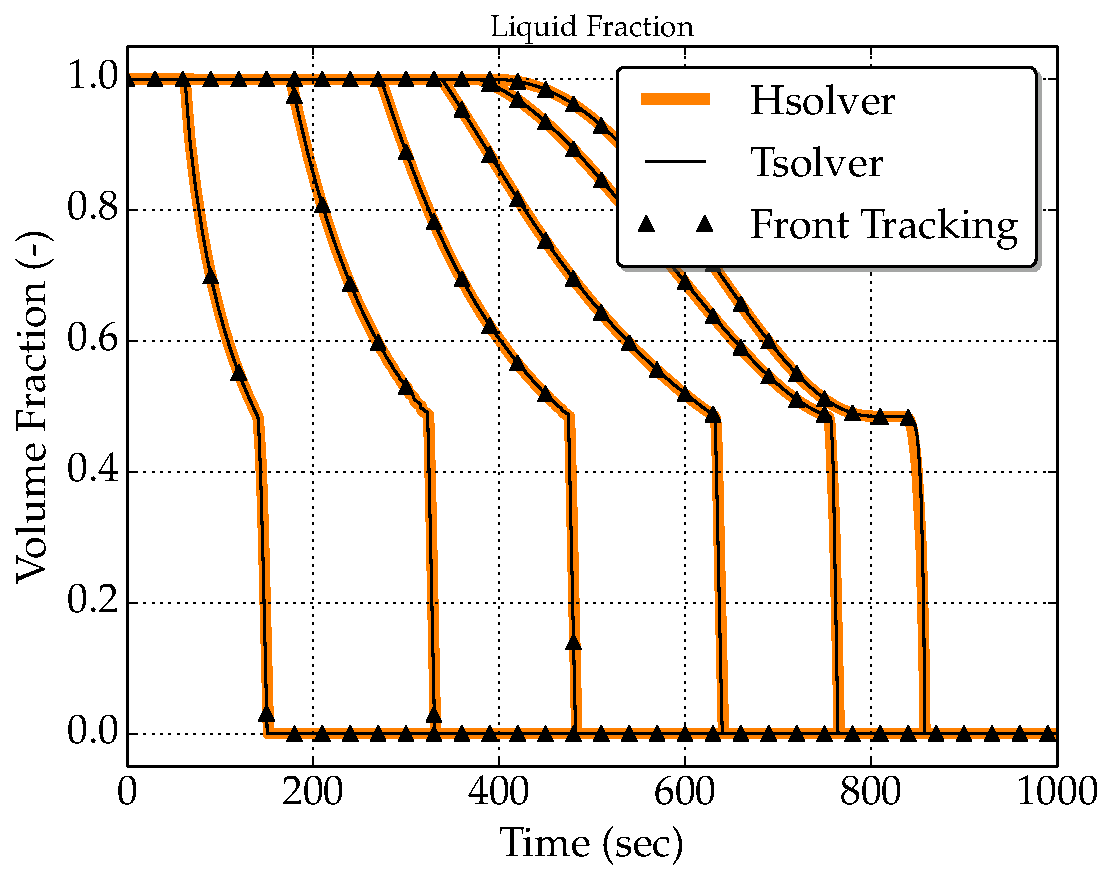
\includegraphics[width=\textwidth]{Chapter2/Graphics/diffusion/diffusion_LF.pdf}
	\caption{}
    \label{fig:validation_diffusion_LF}
  \end{subfigure}
   %------------
\caption{Computed unidirectional heat diffusion during solidification of an \bin{Al}{7}{Si} alloy 
using (orange) the enthalpy method and (black) the temperature method, comparison being made 
for (a) cooling curves  and (b) the liquid fraction history. 
Each curve corresponds to a position along the sample, from 0 cm (cooling 
side) to 10 cm (insulated side), with 2 cm spacing between the positions.} 
\label{fig:validation_diffusion}
\end{figure}
%
%------------------
\subsection{Convection and diffusion}
Conservation equations in \textbf{Table 2} are for mass, momentum and chemical species. 
As for energy, they are presented after the volume averaging technique has been applied 
\citep{ni_volume-averaged_1991, dantzig_solidification_2009}. Moreover, an assumption 
of a static and non deformable solid phase is made. Consequently, the mechanical model is 
reduced to the conservation of momentum in the liquid phase. This assumption also yields 
some other consequences on the mass balance and the liquid momentum conservation. In the 
latter, a Darcy term is added to take into account the dissipative interfacial stress in 
the porous-like mushy zone. Its main parameter is the permeability of the mushy zone, $K$. 
It is considered isotropic, hence reducing to a scalar which is given by the Carman-Kozeny 
relation, based on the secondary dendrite arm spacing $\lambda_2: K= \frac{g^{l^3}  \lambda_2^{2}
 }{180\brac{1-g^l}^2}$. The liquid density being taken constant, its spatial variations 
as a function of temperature and average composition are still needed to compute thermosolutal 
convection forces. For that purpose, the Boussinesq approximation $\rl = \rref \brac{1-\betaT 
\brac{T-\Tref}-\betawl \brac{\wl-\wlref}}$ is used, considering the thermal $\betaT$ and solutal $\betawl$) expansion coefficients 
and a reference density, $\rref$, defined at a reference temperature $\Tref$ and reference 
composition $\wlref$. Values for the references are taken at the liquidus temperature and the nominal 
composition of the alloy, $\w_0$ \citep{carozzani_direct_2013}. More details about the FE formulation can be found in 
the Ph.D work of \citet{rivaux_simulation_2011, carozzani_developpement_2012}. It should be noted that the macroscopic 
solute diffusion coefficient in the solid phase is neglected in \textbf{REF Eq. 15c}. 
%
%----------------------
\begin{figureth}
% textwidth 
{0.9}
%path 
{Chapter2/Graphics/convection_diffusion/smacs_CC.pdf}
% caption
{Experimental cooling curves overlap with the results of the 3D FE convection-diffusion simulation.
The left (LHE) and right (RHE) heat exchangers impose the boundary temperature in the experiment.}
% label
\label{fig:validation_convectiondiffusion}
\end{figureth}
%-----------------------------------
%
The Tsolver’s ability to be coupled with various physical phenomena like macrosegregation and fluid flow 
in porous medium is displayed in this test case. It consists of a solidification benchmark where a \SI{10}{\centi \metre}
width $\times$ \SI{6}{\centi \metre} height $\times$ \SI{1}{\centi \metre} thick cavity containing 
a \bin{Sn}{3}{Pb} melt is cooled down from its two 
narrowest vertical sides using heat exchangers (LHE: left heat exchanger, RHE: right heat exchanger). The 
experiment, inspired by \citet{hebditch_observations_1974} similar set up, has been 
revisited by \citet{hachani_experimental_2012} who performed the solidification with better 
controlled conditions and using an increased number of samples for composition analysis. Recently, a successful 
attempt to simulate the experiment was carried out by \citet{carozzani_direct_2013} relying on an enthalpy resolution. 
All details regarding geometry, finite element discretization, material properties 
and boundary conditions can be found in the latter reference. 
\comment{ I could develop more here giving additional details }
For this computation, solidification paths, phase compositions and phase enthalpies were determined by a thermodynamic 
module dedicated to equilibrium calculations for binary alloys. The 3D simulation results in \textbf{REF Figure 4} show 
a satisfactory agreement with the experimental temperature measurements recorded at mid heights of the cavity and uniformly 
distributed along its width \citep{carozzani_direct_2013}. In fact, simulation results with the Tsolver and the Hsolver were 
found to be almost superimposed, as in \textbf{REF Figure 4}. Regarding the computation, the Tsolver resolution proves to be 
faster than the Hsolver used by \citet{carozzani_direct_2013}: a process time of 7000s required a computation time of 90 hours 
13 minutes compared to 114 hours 21 minutes spent by the enthalpy resolution with 32 cores on the same cluster. The gain factor 
is about 20\%.
